\documentclass[11pt]{article}

\usepackage[margin=1in]{geometry}
\usepackage{amsmath,amssymb}
\usepackage{graphicx}
\usepackage{booktabs}
\usepackage{natbib}
\usepackage{hyperref}
\hypersetup{colorlinks=true, linkcolor=blue, citecolor=blue, urlcolor=blue}

\title{Language Cadence II: A Hybrid Syllable Tokenizer\\ and a Null Result for Periodic Positional Encoding}
\author{Navid Nabijou\thanks{Queen Mary University of London. \texttt{nn333@cantab.ac.uk}}}
\date{October 1, 2026}

\begin{document}
\maketitle

\begin{abstract}
A companion paper (\citeauthor{nabijou2026}, \citeyear{nabijou2026}) tested whether tuning the period of a strictly periodic positional encoding per language improves GPT pretraining, and found a null result traced to a boundary effect -- a purely periodic encoding makes a longer period indistinguishable from a longer usable context -- compounded by a character-level tokenizer, under which a period has no interpretable linguistic meaning. This paper addresses both for English, first building and validating a hybrid syllable tokenizer (CMUdict counts, a spelling-based cut-point algorithm, and an out-of-vocabulary fallback) that we expect to be useful beyond this project wherever English text needs a well-behaved, linguistically grounded syllable-level unit, then adding the periodic component on top of a standard (Vaswani-style) base encoding, which removes the boundary effect directly by keeping absolute-position information available regardless of the period. Sweeping 8 periods with 3 paired seeds each, against a no-periodic baseline and a RoPE control (30 runs, English, syllable-tokenized TED-talk transcripts), we again find a negative result, but of a different character: every periodic configuration underperforms baseline, consistently in direction, yet no individual period is significant after correcting for multiple comparisons. An omnibus test shows the periods differ meaningfully as a group ($p<0.0001$) even though no specific pairwise gap survives correction -- a real effect not resolvable pointwise at this sample size. RoPE outperforms both by a wide margin, confirming the setup can detect a real positional effect. The training curves reveal a further anomaly: the periodic-vs-baseline gap is U-shaped over training, nearly closing mid-run before reopening late, unexplained by anything in the design.
\end{abstract}

\section{Introduction}
\label{sec:intro}

\citet{nabijou2026} set out to test the idea that different natural languages might have an intrinsic ``cadence'' -- a best-performing period for a periodic positional encoding -- by sweeping that period across five languages and reading off whichever period minimized next-token pretraining loss, per language. The result was a clean null, but a diagnosable one: for every language tested, loss decreased monotonically as the period grew, all the way to the model's context length. The paper traced this to what it called the \emph{boundary effect}: because the periodic encoding was the model's \emph{only} source of positional information, a period close to the context length $N$ stops repeating within any single training window, which is functionally equivalent to handing the model a longer usable context -- an improvement with nothing to do with periodicity. The same paper flagged a second, compounding concern without being able to test it: its tokenizer operated at the character level, and a character has no principled relationship to syllable- or clause-level linguistic structure, so a ``period'' measured in characters cannot be interpreted as a period in any unit a genuine rhythmic effect would plausibly operate over.

This paper is a direct sequel addressing both problems, narrowed to a single, more tractable question: for English specifically, does adding a periodic positional-encoding component on top of a normal positional encoding improve training efficiency, as measured by test loss at a fixed training budget? (The companion paper instead compared a per-language optimum across five languages.) Two design changes follow directly from the companion paper's diagnosis. First, the periodic component is now added on top of a fixed, standard (Vaswani-style) base positional encoding, so that full absolute-position information is always available to the model regardless of the chosen period -- this removes the mechanism behind the boundary effect at the architectural level. In the companion paper, the periodic encoding was the model's only positional signal; here it is strictly additional, and the removal is architectural rather than a statistical control. Second, we build a dedicated hybrid syllable tokenizer for English, so that a candidate period corresponds to a linguistically motivated unit, the syllable. The companion paper tokenized at the character level, an orthographic unit with no principled relationship to syllable structure.

The tokenizer is, in our view, as substantial a contribution of this project as the positional-encoding experiment itself, and we give it a correspondingly detailed treatment in Section~\ref{sec:tokenizer}: its design, its validation against CMUdict ground truth, and the vocabulary built from it. Although it was built to give the period sweep an interpretable unit, nothing about its design is specific to that purpose, and it may be of independent interest for other English NLP work that wants a syllable-level granularity -- phonologically or prosodically motivated modeling, text-to-speech front ends, or readability and rhythm analysis among them. Section~\ref{sec:method} describes the rest of the experimental method -- the positional-encoding design, the dataset, and the sweep -- and Section~\ref{sec:experiments} reports the results, including a formal statistical analysis addressing a question any reader of a sweep plot should ask: is the period-to-period structure visible in the data distinguishable from noise, or is it an artifact of how the plot happens to be scaled? Section~\ref{sec:discussion} offers deliberately labeled speculation about what might be driving the negative result and its internal structure, and Section~\ref{sec:limitations} states the caveats and open questions plainly.

\section{Tokenizer}
\label{sec:tokenizer}

Character-level tokenization treats every language identically regardless of its structure, which is attractive for cross-linguistic comparison but was identified in the companion paper as a likely reason the periodic-encoding idea was never given a fair test: a period expressed in characters is not interpretable as a period in any unit a rhythmic effect would plausibly operate over, since a fixed number of characters corresponds to a different amount of linguistic structure depending on orthographic depth (compare English ``th'' or German ``sch'', each one phoneme spelled with two characters, to a language with a shallower orthography). The natural unit to test the cadence hypothesis against is instead something closer to the syllable. (The mora is a finer-grained unit in the general prosodic hierarchy, and is the relevant rhythmic unit for mora-timed languages such as Japanese, but it plays no comparable role in English phonology -- so for an English-only tokenizer, the syllable is the finest unit that is actually doing linguistic work.) Standard subword tokenizers (byte-pair encoding and its relatives) were ruled out for the same reason as the character-level choice: their piece boundaries are chosen to minimize a compression objective, not to track any linguistic unit, so a period measured in BPE pieces would carry exactly the same interpretability problem the companion paper diagnosed.

We therefore built a dedicated \emph{hybrid syllable tokenizer} for English: a piece boundary placement that is anchored to a genuine linguistic count (dictionary syllable counts) wherever that ground truth is available, with a validated fallback where it is not.

\subsection{Design}

The tokenizer operates on lowercased text and produces a flat stream of pieces: one or more syllable pieces per word (the first piece of each word carries a leading marker \texttt{\_}, so word boundaries are always recoverable from the piece stream alone), with punctuation characters and single digits emitted as standalone pieces. Syllabifying a single word proceeds in two stages.

\textbf{Syllable count.} For a word present in the CMUdict pronunciation dictionary \citep{cmudict}, the syllable count $k$ is the number of vowel phones in its pronunciation (CMUdict phones are stress-marked, so a phone's syllabicity is read directly off a trailing digit). Roughly 1.9\% of CMUdict entries have more than one listed pronunciation with disagreeing counts; we resolve this by majority vote across pronunciations, breaking ties in favor of the first-listed one. For words absent from CMUdict -- out-of-vocabulary (OOV) with respect to the dictionary, about 1.6\% of word tokens in our evaluation corpus -- $k$ is instead estimated by a fallback: majority vote across a vowel-group heuristic (count maximal runs of vowel letters) and the syllable counts implied by two independent automatic syllabifiers, \texttt{pyphen} \citep{pyphen} and NLTK's Sonority Sequencing Principle (SSP) tokenizer \citep{nltksyl}.

\textbf{Cut placement.} Given $k$, the word's $k-1$ internal cut points are chosen from the $L-1$ inter-letter boundaries of an $L$-letter word by a dynamic program that scores each candidate boundary set by: agreement with \texttt{pyphen}'s own hyphenation points; agreement with the SSP splitter's boundaries; a bonus when the syllable immediately following a cut begins with a licensed English consonant cluster (a fixed allow-list of legal onsets, e.g. \emph{bl-}, \emph{str-}, \emph{th-}); and small bonuses for a handful of common morphological suffix boundaries (\emph{-ing}, \emph{-tion}, \emph{-ment}, and similar). Two classes of word are special-cased rather than left to the general scoring: contractions, where a clitic (\emph{n't}, \emph{'s}, \emph{'ll}, \ldots) is split off as its own final piece (\emph{didn't} $\to$ \emph{did-n't}); and words ending in a consonant plus syllabic \emph{-le} (\emph{-ble}, \emph{-cle}, \emph{-dle}, \ldots), where that ending is treated as a syllable nucleus in its own right even though it contains no written vowel (\emph{enabling} $\to$ \emph{en-a-bl-ing}).

This design was deliberately chosen over either automatic syllabifier alone. On a held-out evaluation sample (the Brown corpus; see Section~\ref{sec:tokenizer-validation}), \texttt{pyphen} alone matches CMUdict's syllable \emph{count} for only 79.3\% of out-of-vocabulary-probe words and NLTK's SSP splitter is weaker still, since each tool encodes a different, imperfect model of English syllabification (\texttt{pyphen} under-splits short words; SSP over-splits silent-\emph{e} words such as \emph{time} or \emph{have}). Anchoring the \emph{count} to CMUdict wherever possible, and only falling back to a vote among the automatic tools where CMUdict has no entry, removes most of this disagreement by construction for the 98.4\% of word tokens CMUdict does cover.

\subsection{Validation}
\label{sec:tokenizer-validation}

We evaluate the tokenizer on the Brown corpus (991{,}429 word tokens, 42{,}256 distinct word types), which is independent of both the training corpus used for the main experiment (Section~\ref{sec:dataset}) and of CMUdict itself. Table~\ref{tab:tokenizer-eval} summarizes the key statistics.

\begin{table}[h]
\centering
\caption{Hybrid syllable tokenizer, evaluated on the Brown corpus.}
\label{tab:tokenizer-eval}
\begin{tabular}{lr}
\toprule
Quantity & Value \\
\midrule
CMUdict coverage (word tokens) & 98.4\% \\
CMUdict coverage (distinct word types) & 87.8\% \\
Pieces rejoin the original word & 100.0\% \\
Words with a vowel letter in every piece & 98.4\% \\
Mean syllables per word & 1.56 \\
Mean characters per syllable piece & 3.03 \\
Fallback syllable-count accuracy (OOV probe) & 83.0\% \\
\quad vs.\ \texttt{pyphen} alone & 79.3\% \\
\bottomrule
\end{tabular}
\end{table}

By construction, the pieces always concatenate back to the original word, so the first row after dictionary coverage is guaranteed rather than measured; it is included as a sanity check that the implementation has no silent bugs. (The next row, vowel-in-every-piece, is a genuinely measured quantity -- piece counts summing to exactly $k$ does not guarantee every piece contains a vowel letter, which is why it falls short of 100\%.) The more informative numbers are coverage (how often the gold-standard count is even available) and fallback accuracy (how good the estimate is when it is not): the fallback -- majority vote across three independent estimators -- outperforms the best single automatic syllabifier (\texttt{pyphen}) by 3.7 points on words deliberately treated as out-of-vocabulary for the purpose of this probe, despite \texttt{pyphen} being one of the fallback's three voters, confirming that combining signals is worth the added complexity. The weakest statistic we measured is agreement with \texttt{pyphen}'s specific \emph{cut positions} (as opposed to syllable \emph{counts}) on the subset of words where both tools agree on the count: only 60.1\% of such words receive identical cut placement from the two methods. We read this as expected rather than concerning -- when the count is already fixed, the DP's additional scoring terms (legal-onset and suffix bonuses, not used by \texttt{pyphen}) are free to move the cut to a linguistically better-justified position than \texttt{pyphen}'s own heuristic, and we have no independent ground truth for cut \emph{placement} (as opposed to count) with which to adjudicate between them; we report the discrepancy for transparency rather than treating either tool as gold-standard here.

\subsection{Vocabulary}

A piece vocabulary was built directly from the training split of the dataset described in Section~\ref{sec:dataset} (6{,}398{,}658 training pieces, 19{,}286 distinct piece types), by frequency rank, with out-of-vocabulary pieces falling back to a character-level encoding so that no input is ever unrepresentable. Figure~\ref{fig:vocab-coverage} shows coverage as a function of vocabulary size on both the training split itself and the held-out validation split. We fixed the vocabulary at 8{,}000 pieces, which covers 99.5\% of training tokens and 99.2\% of held-out validation tokens -- past this point the coverage curve has visibly flattened, and the training-time cost of a larger output layer is not justified by the small additional coverage available (vocabulary sizes above 16{,}000 approach 100\% coverage but at roughly double the parameter cost in the model's embedding and output layers).

\begin{figure}[h]
\centering
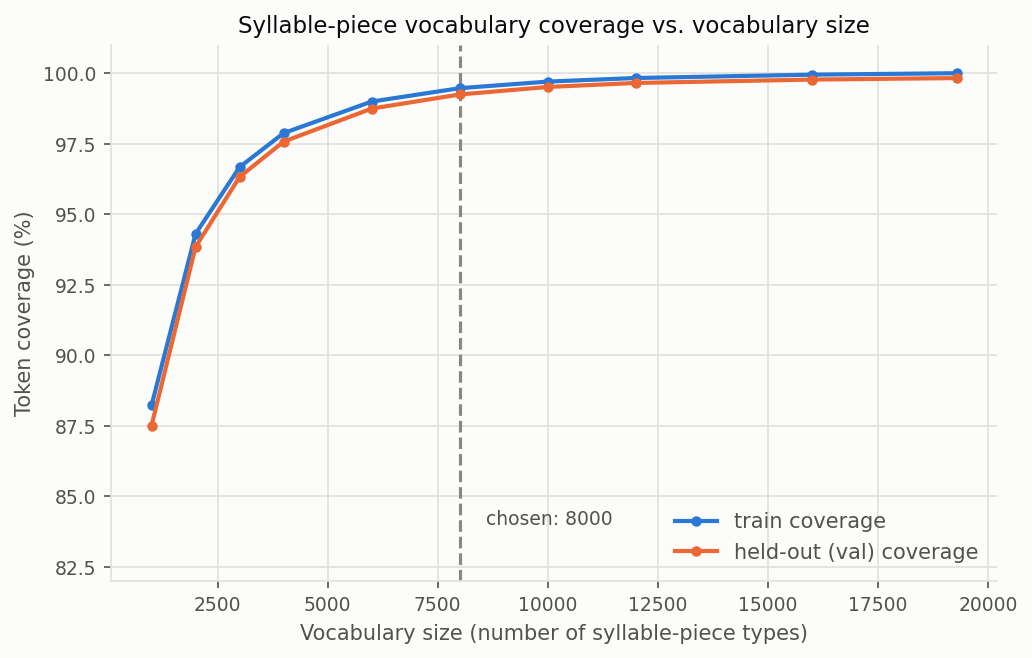
\includegraphics[width=0.75\textwidth]{figures/vocab_coverage_curve.png}
\caption{Syllable-piece vocabulary coverage as a function of vocabulary size, measured on the training split (used to build the vocabulary) and the held-out validation split. The chosen size, 8{,}000 pieces, is marked.}
\label{fig:vocab-coverage}
\end{figure}

\subsection{Known weaknesses}

Three limitations of the tokenizer are worth stating plainly, since they bear directly on how the main experiment's results should be interpreted (Section~\ref{sec:limitations} returns to each). First, CMUdict reflects General American pronunciation; TED speakers are drawn from many English varieties, so the dictionary's syllable counts are not uniformly accurate ground truth for every speaker's actual pronunciation, even where a word is covered. Second, the tokenizer counts \emph{canonical} dictionary syllables, not syllables as they were actually realized in any given utterance -- connected speech routinely elides or merges syllables in ways no dictionary look-up can capture. Third, cut-\emph{placement} (as opposed to count) is validated only by agreement with other heuristic tools, not against any independent ground truth, as noted above. None of these affects the syllable \emph{counts} that ultimately determine the piece stream's granularity -- the quantity most relevant to testing a periodic-encoding hypothesis -- but they mean the tokenizer should be read as a substantially more linguistically grounded unit than characters or BPE pieces, not as a perfect phonetic transcription. With that caveat, these limitations are modest relative to what character- or BPE-level tokenization offers in the way of syllable awareness, which is essentially none, so the tokenizer should still be a useful building block for other syllable-aware work on English, independent of the periodic-encoding question it was built to serve here.

\section{Method}
\label{sec:method}

\subsection{Positional encoding}
\label{sec:pe-method}

As in the companion paper, each position $n \in \{0, \ldots, N-1\}$ is encoded by a $D$-dimensional vector built from $H = D/2$ sine/cosine row-pairs, and the periodic component is constructed so that it has an exact period $P$: row-pair $j$ ($j = 1, \ldots, H$) is assigned the folded harmonic
\[
k_j = \min\big(j \bmod P,\; P - (j \bmod P)\big),
\]
which avoids wasting embedding capacity on harmonics that would otherwise alias (fold back onto an earlier one, up to sign) once $j$ exceeds $P/2$; see \citet{nabijou2026} for the derivation. With this assignment, the periodic component $\boldsymbol{\Pi}_{\text{per}}$ has entries
\[
\boldsymbol{\Pi}_{\text{per}}[2j-2, n] = \sin\!\left(\frac{2\pi k_j n}{P}\right), \qquad
\boldsymbol{\Pi}_{\text{per}}[2j-1, n] = \cos\!\left(\frac{2\pi k_j n}{P}\right).
\]

The crucial difference from the companion paper is what this periodic component is combined with. There, $\boldsymbol{\Pi}_{\text{per}}$ was the model's \emph{entire} positional signal, which is precisely what allowed a long period to masquerade as extra usable context (Section~\ref{sec:intro}). Here, we first compute a standard, fixed, non-periodic base encoding $\boldsymbol{\Pi}_{\text{base}}$ -- the geometric frequency spread of \citet{vaswani2017}, with entries $\boldsymbol{\Pi}_{\text{base}}[2i, n] = \sin(n / 10000^{2i/D})$ and $\boldsymbol{\Pi}_{\text{base}}[2i+1, n] = \cos(n / 10000^{2i/D})$ -- and form the combined encoding
\[
\boldsymbol{\Pi}(n) = \boldsymbol{\Pi}_{\text{base}}(n) + \boldsymbol{\Pi}_{\text{per}}(n; P).
\]
Because $\boldsymbol{\Pi}_{\text{base}}$ is present regardless of $P$, the model always has access to full absolute-position information; the periodic component can only ever add to that, never substitute for it. This directly removes the mechanism behind the boundary effect: a large $P$ no longer corresponds to ``more usable context,'' since the base encoding already supplies a usable context signal of its own, constant across the sweep. A \emph{no-periodic-component} configuration -- $\boldsymbol{\Pi}(n) = \boldsymbol{\Pi}_{\text{base}}(n)$ alone -- serves as the baseline against which every periodic configuration is compared (Section~\ref{sec:sweep}).

$\boldsymbol{\Pi}(n)$ is injected by concatenating it with the token embedding and passing the result through a learned linear projection back to $D$ dimensions, $\mathbf{x} = \text{Linear}(\text{concat}(\mathbf{e}_{\text{tok}}, \boldsymbol{\Pi}))$. We chose concatenation over additive injection following a calibration pilot in the companion paper's own project, which found that additive injection has a narrow, saturating useful amplitude range in a pre-norm transformer: every block here opens with LayerNorm, and $\text{LayerNorm}(c\mathbf{v}) = \text{LayerNorm}(\mathbf{v})$ for any positive scalar $c$, so past a small amplitude threshold the positional signal's relative contribution is clamped regardless of how large it is made. Concatenation sidesteps this fragility at the cost of one extra learned projection layer, with no amplitude hyperparameter to tune. We use it for every configuration in the sweep below, including the baseline, so injection method is held fixed and cannot confound the comparison.

As a stronger positional-encoding control, we also train a \emph{rotary position embedding} (RoPE) configuration \citep{su2021roformer}. RoPE conveys position by rotating the query and key vectors inside each attention head, by an angle that is a function of relative position, before the attention dot product is computed -- a structurally different mechanism that acts directly on what attention can represent. It is included as a positive control: a configuration already well established as effective, included to confirm that the overall pipeline (architecture, data, training protocol) is capable of detecting a real positional-encoding effect when one is present. We do not use it to test the periodicity hypothesis itself.

\subsection{Dataset}
\label{sec:dataset}

Training data is the English source side of the WIT3/IWSLT TED-talk transcript collection \citep{cettolo2012wit3}, 2016 release: 2{,}085 talks spanning three decades, giving $4.3$M words before preprocessing. Talks were processed by stripping parenthetical audience and audio cues (``(Laughter)'', ``(Applause)'', and 14{,}631 similar occurrences across the corpus), dropping the 11 talks remaining under 100 words after cleaning (near-wordless music or dance performances), and keeping casing, punctuation, and digits as written. The corpus was split by \emph{speaker}, greedily balanced to a 90/5/5 word-count split with zero speaker overlap verified between splits. A talk-level split would have leaked a speaker's idiosyncratic vocabulary and style across the train/test boundary, since 221 of the corpus's 1{,}767 distinct speakers give more than one talk. The resulting splits are 1{,}667 talks / 3.89M words / 1{,}363 speakers (train), 202 talks / 216k words / 197 speakers (validation), and 205 talks / 216k words / 198 speakers (test).

\subsection{Architecture}

The architecture is held fixed across every configuration in the sweep: embedding dimension $D = 128$, $H = 64$ positional-encoding row-pairs, 4 transformer layers, 4 attention heads (head dimension 32), context length $N = 1{,}024$, and the 8{,}000-piece syllable vocabulary of Section~\ref{sec:tokenizer} -- approximately 2.87M parameters in total. This is a deliberately small, laptop-scale model; Section~\ref{sec:limitations} returns to what that implies for the results.

\subsection{Sweep design and protocol}
\label{sec:sweep}

The period is swept over
\[
P \in \{2, 3, 6, 9, 16, 45, 128, 1024\},
\]
reallocated toward the low end relative to the companion paper's more evenly log-spaced grid, on linguistic grounds: these values span roughly the scale of a syllable, a short word, and a phrase, which is the range at which a genuine rhythmic effect operating on syllable-tokenized text would plausibly appear. $P=128$ is retained as the companion paper's geometric-distinguishability optimum for $H=32$ (that paper's row-pair count; see its Section~2.1), included here as a direct cross-paper comparison point even though $H=64$ in this paper's own architecture shifts where that optimum would actually fall. $P=1{,}024 = N$ is retained specifically as the boundary-effect check described in Section~\ref{sec:pe-method}: with a base encoding now always present, this is the direct test of whether that companion paper's monotonic-to-the-boundary pattern persists once the mechanism behind it has been architecturally removed. $P=45$ fills the resulting gap between the low cluster and $P=128$.

Each of the 8 periodic configurations, plus the no-periodic baseline and the RoPE control, was trained with 3 random seeds -- and critically, the \emph{same} three seeds (identical parameter initialization and identical training-data shuffle order) are reused across all 10 configurations. This makes every pairwise comparison between two configurations a \emph{paired} one (seed-matched), which removes seed-to-seed noise common to both arms of any given comparison and substantially increases statistical power at a fixed, small number of seeds (Section~\ref{sec:stats}). In total this gives $8 \times 3 + 3 + 3 = 30$ training runs.

Each run trains for 3{,}000 steps at batch size 16 and a single fixed learning rate, corresponding to roughly 7--8 passes over the 3.89M-word training split. Validation loss on a fixed evaluation subset is tracked every 100 steps throughout training (Section~\ref{sec:training-dynamics}). The checkpoint with the lowest such validation loss over the whole run is the one evaluated on the full held-out test set and reported as that run's result; this guards against the overfitting risk a 7--8-pass budget invites. For the headline comparison between periods (Section~\ref{sec:headline}), the single best-performing period is selected using validation loss alone, so no part of the headline comparison is chosen by looking at the test set.

\section{Experiments}
\label{sec:experiments}

All 30 runs completed without incident: no run diverged (checked against a hard non-finite-loss halt) or triggered a soft loss-spike warning, and every run reached its full 3{,}000-step budget. We report results in three parts: the headline test-loss comparison (Section~\ref{sec:headline}), a formal statistical analysis of that comparison (Section~\ref{sec:stats}), and an analysis of how loss evolves \emph{during} training rather than only where it ends up (Section~\ref{sec:training-dynamics}).

\subsection{Headline comparison}
\label{sec:headline}

Table~\ref{tab:headline} and Figure~\ref{fig:period-sweep} report mean test loss (cross-entropy, nats per syllable-piece\footnote{This paper tokenizes at the syllable-piece level; the companion paper tokenized at the character level. Loss values here are therefore not directly comparable to that paper's reported nats-per-character figures -- a syllable piece carries, on average, 3.03 characters' worth of information (Table~\ref{tab:tokenizer-eval}), so the two loss scales measure different-sized prediction units.}, at the best-validation-loss checkpoint) across the 3 seeds for each of the 10 configurations.

\begin{table}[h]
\centering
\caption{Mean test loss by configuration (3 seeds each, mean $\pm$ standard deviation).}
\label{tab:headline}
\begin{tabular}{lr}
\toprule
Configuration & Test loss \\
\midrule
Baseline (no periodic component) & $3.9411 \pm 0.0165$ \\
Periodic, $P=2$ & $3.9641 \pm 0.0042$ \\
Periodic, $P=3$ & $3.9573 \pm 0.0029$ \\
Periodic, $P=6$ & $3.9611 \pm 0.0049$ \\
Periodic, $P=9$ & $3.9625 \pm 0.0065$ \\
Periodic, $P=16$ & $3.9648 \pm 0.0044$ \\
Periodic, $P=45$ & $3.9814 \pm 0.0042$ \\
Periodic, $P=128$ & $3.9959 \pm 0.0073$ \\
Periodic, $P=1024$ & $3.9825 \pm 0.0078$ \\
RoPE & $3.6141 \pm 0.0068$ \\
\bottomrule
\end{tabular}
\end{table}

\begin{figure}[h]
\centering
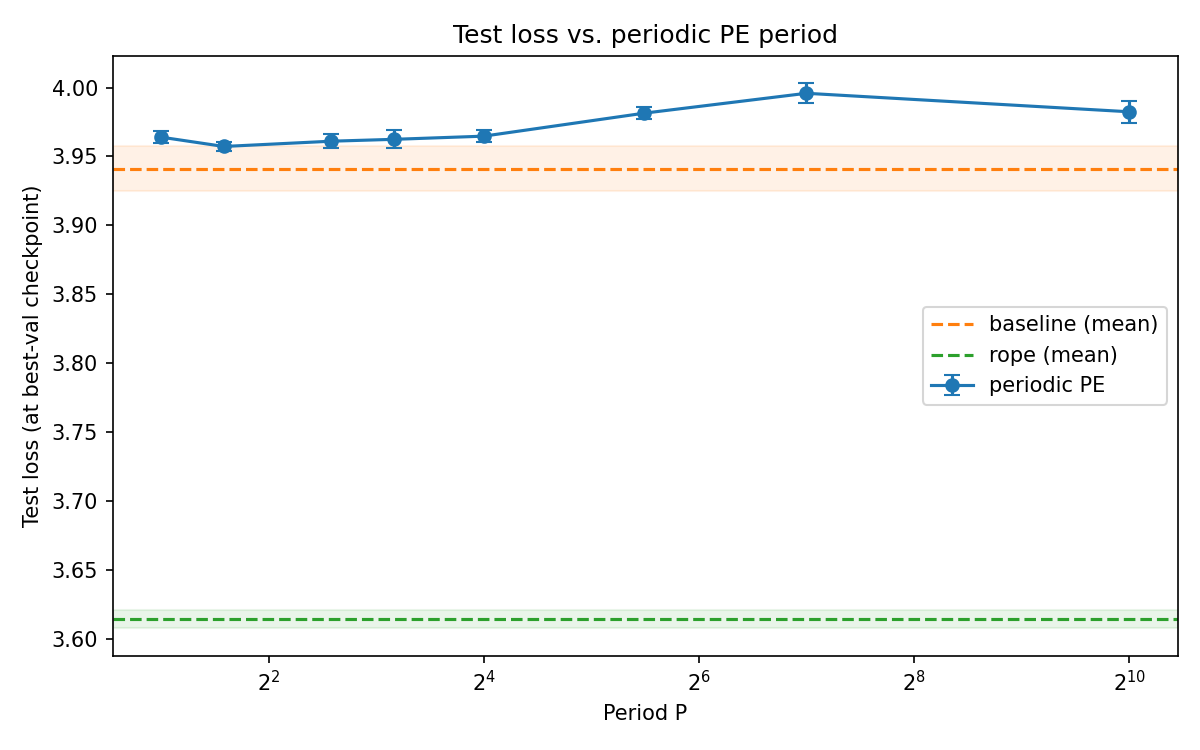
\includegraphics[width=0.8\textwidth]{figures/period_sweep.png}
\caption{Test loss vs.\ period $P$ (log-$x$), with the no-periodic baseline and RoPE shown as reference bands (mean $\pm$ 1 std.). Every periodic configuration lies above the baseline; RoPE lies well below both.}
\label{fig:period-sweep}
\end{figure}

Every one of the 8 periodic configurations is worse than the baseline, with the best (validation-selected) period at $P=3$, matching the period selected by test loss as well -- the two selection criteria agree, which rules out the specific concern that a best-period claim here would reflect test-set peeking. RoPE is a large, unambiguous win over both: a 0.33-nat gap to baseline, roughly an order of magnitude larger than any periodic-vs-baseline gap observed. We treat the RoPE comparison purely as the positive control described in Section~\ref{sec:pe-method} -- its advantage over additive/concatenative positional encodings is already well established in the literature \citep{su2021roformer} and is not itself a finding of this paper -- and do not analyze it further below.

The pattern across periods is not monotonic: the four smallest periods ($P \in \{2,3,6,9,16\}$) cluster closely together and perform best among the periodic configurations; $P=45$ and especially $P=128$ are the worst points on the grid; $P=1{,}024=N$ partially, but not fully, recovers. This is qualitatively different from the companion paper's result, where loss decreased monotonically all the way to $P=N$ in every language with no exception -- here, $P=N$ is not the best point, and the boundary-effect mechanism's signature (a period approaching $N$ always winning) is absent. Section~\ref{sec:stats} asks how much of this shape can actually be trusted statistically.

\subsection{Statistical analysis}
\label{sec:stats}

A sweep plot with 8 points invites two questions a reader should not take on faith: is any individual period's apparent disadvantage relative to baseline real, or within the range small-sample noise would produce; and is the period-to-period shape visible in Figure~\ref{fig:period-sweep} a genuine effect, or just how the data happens to look at this particular scale? We address both directly, exploiting the paired-seed design of Section~\ref{sec:sweep} throughout.

\textbf{Periodic vs.\ baseline.} For each of the 8 periods, we run a paired $t$-test (seed-matched) against the baseline, and apply Holm--Bonferroni correction \citep{holm1979} across the resulting family of 8 comparisons to control the family-wise error rate. Table~\ref{tab:stats} reports the results, together with Cohen's $d_z$ (the paired effect size: mean of the paired differences divided by their standard deviation).

\begin{table}[h]
\centering
\caption{Periodic vs.\ baseline, paired $t$-test with Holm--Bonferroni correction across the 8 comparisons.}
\label{tab:stats}
\begin{tabular}{lrrrrr}
\toprule
$P$ & Mean diff.\ & $t$ & $p$ (raw) & $p$ (Holm) & Cohen's $d_z$ \\
\midrule
2 & $+0.0230$ & 2.44 & 0.1348 & 0.4345 & 1.41 \\
3 & $+0.0162$ & 2.03 & 0.1791 & 0.4345 & 1.17 \\
6 & $+0.0200$ & 3.00 & 0.0954 & 0.4345 & 1.73 \\
9 & $+0.0214$ & 3.58 & 0.0700 & 0.4203 & 2.07 \\
16 & $+0.0237$ & 3.17 & 0.0869 & 0.4345 & 1.83 \\
45 & $+0.0404$ & 5.35 & 0.0332 & 0.2656 & 3.09 \\
128 & $+0.0548$ & 4.44 & 0.0471 & 0.3296 & 2.57 \\
1024 & $+0.0414$ & 3.13 & 0.0888 & 0.4345 & 1.81 \\
\bottomrule
\end{tabular}
\end{table}

No individual period's disadvantage survives correction at $\alpha = 0.05$: even the best uncorrected case ($P=45$, raw $p=0.033$) is corrected to $p=0.27$. At the same time, all 8 comparisons point in the same direction (periodic always worse) with uniformly large paired effect sizes ($d_z$ from 1.17 to 3.09) -- a pattern more consistent with a real but small effect that 3 seeds and an 8-way correction simply lack the power to confirm individually, than with there being no effect at all. We report it accordingly: probably real, not formally established at this sample size.

\textbf{Is the period-to-period shape real?} We next ask whether the 8 periodic configurations differ meaningfully \emph{from one another}, using two omnibus tests that treat period as a within-subject factor and seed as the subject: a repeated-measures ANOVA and a Friedman test (a non-parametric cross-check, appropriate given only 3 observations per cell). Both reject the null of no period effect decisively: $F(7,14) = 21.62$, $p < 10^{-5}$ (RM-ANOVA); $\chi^2 = 19.0$, $p = 0.0082$ (Friedman). Because each test's error term is the seed-by-period residual variance, this is a direct comparison of the period-to-period spread against exactly the noise that varying the random seed produces -- so the answer to ``is this shape just an artifact of the plot's scale'' is no: the spread in Figure~\ref{fig:period-sweep} is larger than seed noise alone would produce, at high confidence.

This does not, however, mean every visually apparent feature of the curve is individually confirmed. We computed all $\binom{8}{2}=28$ pairwise period-vs-period comparisons and Holm-corrected across that full family, including the comparison between the single best period ($P=3$) and the single worst ($P=128$) -- the largest gap on the grid. Naively testing only that pre-selected extreme pair, uncorrected, gives $p=0.0155$; but because that pair was selected \emph{by looking at the data} (the lowest and highest of 8 means), an uncorrected test on it is invalid -- this is the same ``testing the winner'' problem that motivates using a corrected procedure such as Tukey's HSD rather than an ordinary $t$-test when comparing the extremes of several groups. Correcting properly, across the full 28-pair family the best-vs-worst comparison is not significant ($p_{\text{Holm}}=0.34$).

Taken together: the omnibus test establishes that real, non-noise structure exists across the 8 periods (a result that pools all the data into a single decision); no specific pairwise comparison between periods, including the largest one, is individually confirmed once properly corrected for having been selected from the data (a much narrower claim, with far less statistical power at $n=3$). This is a standard and well-documented statistical pattern rather than a contradiction -- an omnibus test is routinely more powerful than its own post-hoc pairwise comparisons -- but it means the specific shape described at the end of Section~\ref{sec:headline} (low periods clustering, $P=45/128$ worst, partial recovery at $P=1{,}024$) should be read as a visually suggestive, probably-real pattern rather than a set of individually established facts. More seeds would be needed to say with confidence which specific periods differ from which.

\subsection{Training dynamics}
\label{sec:training-dynamics}

The comparisons above are all evaluated at a single point: the best-validation-loss checkpoint of a finished run. We separately examined how the periodic-vs-baseline gap evolves \emph{during} training, using the validation loss tracked every 100 steps (Section~\ref{sec:sweep}). Figure~\ref{fig:training-curves} shows all 10 configurations' validation loss against training step; Figure~\ref{fig:training-curves-periodic} isolates the periodic configurations and baseline on their own scale, since RoPE's much larger gap otherwise compresses the more subtle structure of interest.

\begin{figure}[h]
\centering
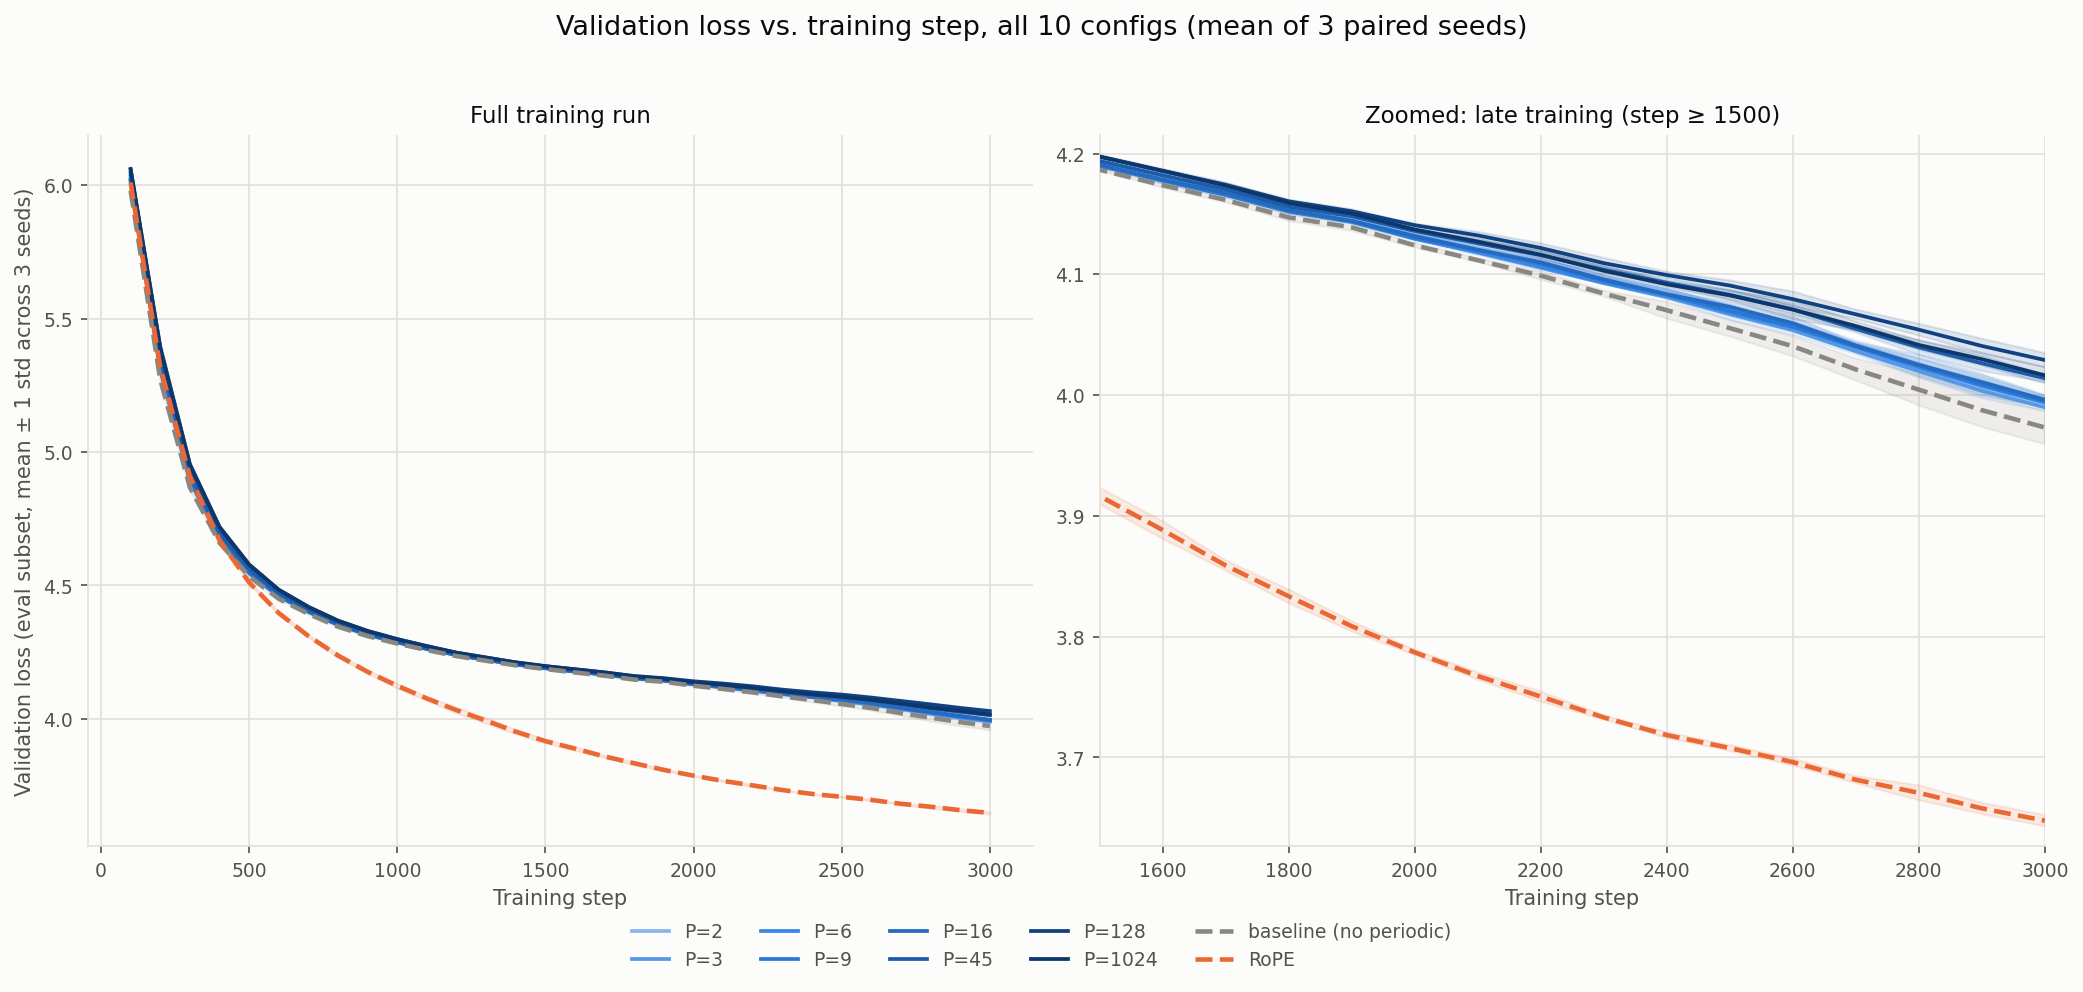
\includegraphics[width=\textwidth]{figures/training_curves.png}
\caption{Validation loss vs.\ training step, all 10 configurations (mean of 3 paired seeds). Right: zoomed to the back half of training.}
\label{fig:training-curves}
\end{figure}

\begin{figure}[h]
\centering
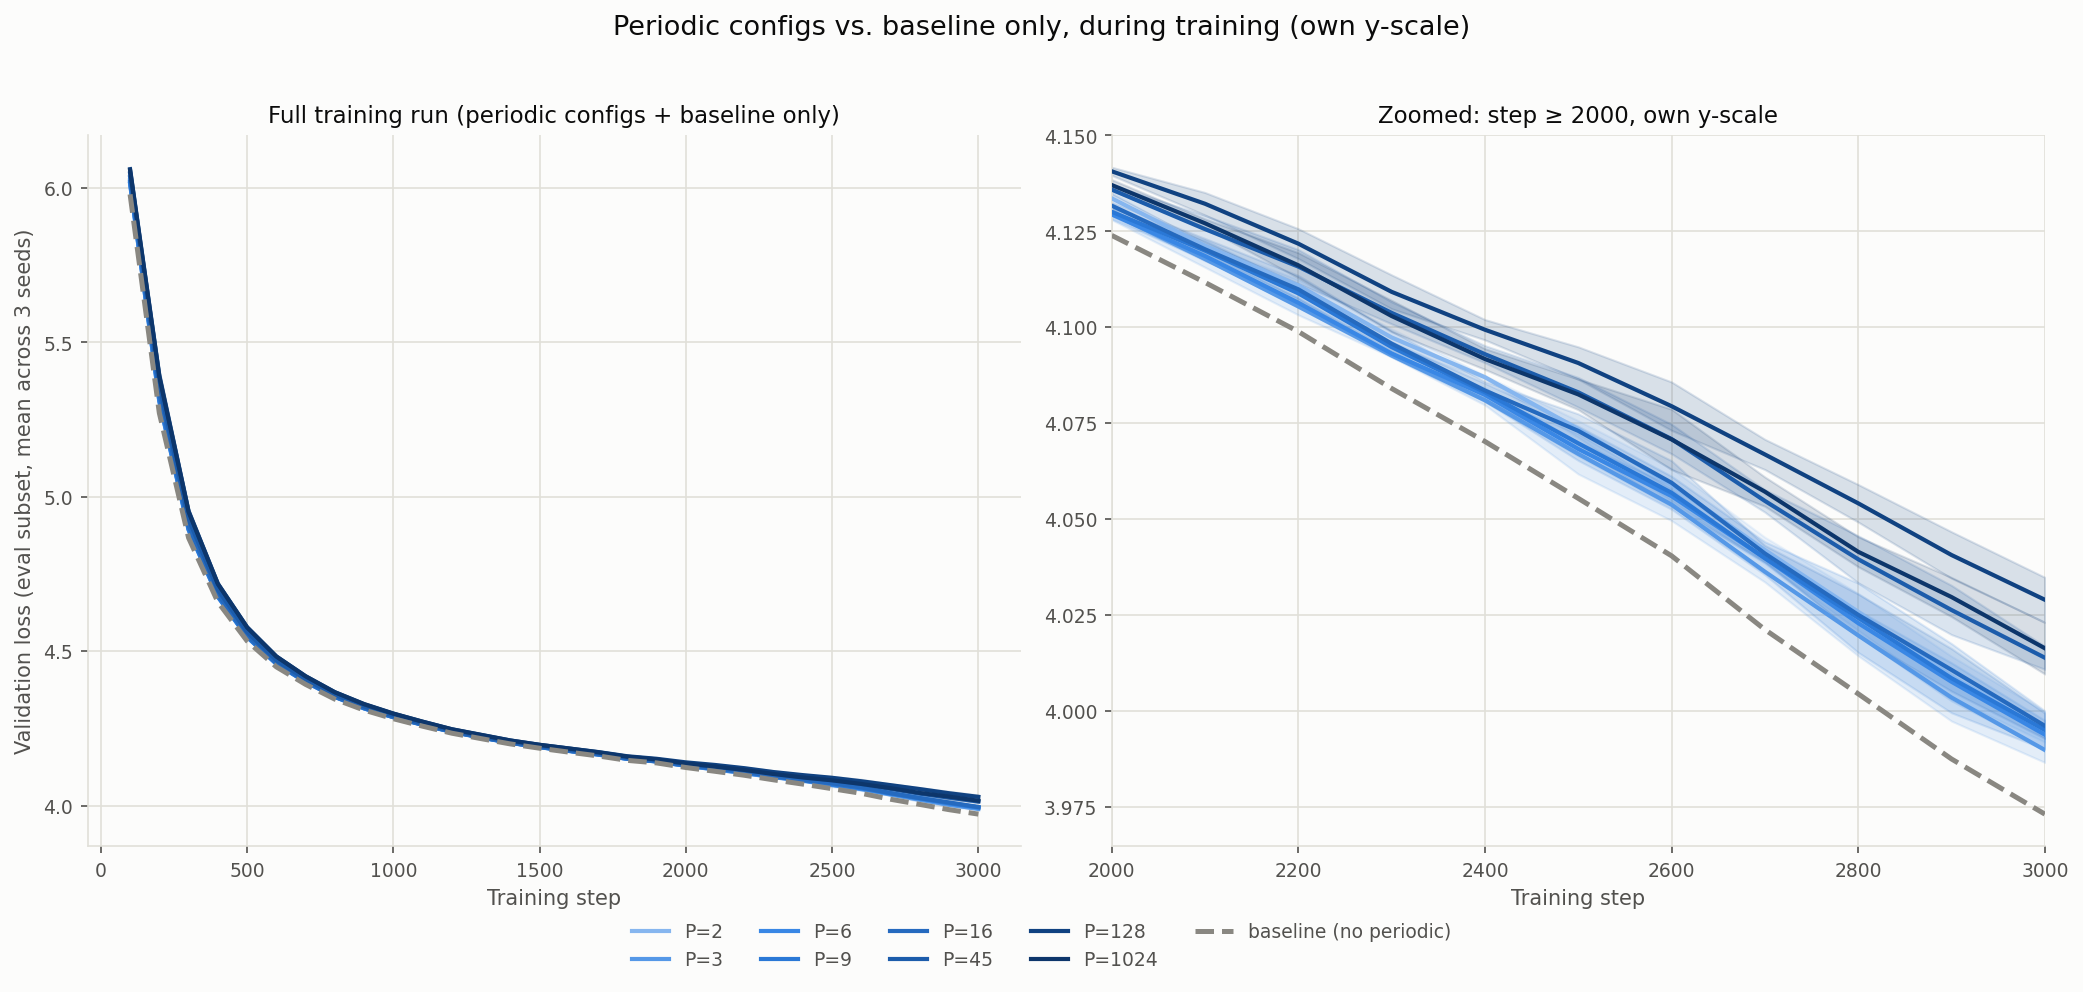
\includegraphics[width=\textwidth]{figures/training_curves_periodic_only.png}
\caption{Periodic configurations and baseline only, on their own $y$-scale. Right: zoomed to step $\geq 2{,}000$.}
\label{fig:training-curves-periodic}
\end{figure}

No training instability is visible in either plot -- every curve is smooth and monotonically decreasing, consistent with the complete absence of divergence or loss-spike events across all 30 runs (Section~\ref{sec:experiments}). A more specific pattern is visible instead: the periodic-vs-baseline gap is not constant over the course of training, but \emph{U-shaped}. Measuring the mean periodic configuration's validation loss minus the baseline's at each tracked step, the gap starts at 0.055 at step 100 (dominated by early optimization noise), shrinks steadily through the first $\sim$1{,}500 steps (roughly 2--3 of the run's 7--8 epochs) to a minimum of 0.006 -- essentially indistinguishable from baseline -- and then reopens, growing back to 0.030 by step 2{,}900, close to where the final-checkpoint comparison in Section~\ref{sec:headline} finds it. The spread \emph{among} the 8 periodic configurations shows the identical shape (0.047 at step 100, down to 0.008 at step 1{,}500, back up to 0.037 by step 2{,}900).

This is, to our knowledge, a new and unexplained observation: the periodic-vs-baseline disadvantage is specifically a late-training phenomenon. It does not look like a from-the-start optimization-speed penalty -- the periodic and baseline models are nearly indistinguishable in the middle of training and only diverge again in the final epochs. We return to what might explain this in Section~\ref{sec:discussion}. The obvious direct follow-up, examining the train/validation loss gap per configuration to check whether periodic configurations show disproportionate late-epoch overfitting, is flagged as future work (Section~\ref{sec:conclusion}).

\section{Discussion}
\label{sec:discussion}

This section is explicitly speculative. None of the mechanisms proposed here were tested directly; we label them as candidate explanations for the patterns in Section~\ref{sec:experiments}, worth stating plainly rather than leaving the results unexplained, but not to be read as established findings.

\subsection{Why might the periodic component underperform baseline?}

A priori, there is no reason the periodic component had to hurt: it could instead have supplied a useful inductive bias and sped up training, since nothing about adding an extra, cheaply-computed positional feature is obviously harmful. The fact that every periodic configuration underperforms baseline (Section~\ref{sec:headline}) shows that if such a beneficial bias exists, it is outweighed by other effects. We consider three candidate mechanisms, in order of how directly they bear on the net-negative result:

\begin{enumerate}
\item \textbf{Integration cost under a fixed training budget.} Concatenation injection adds a larger learned projection than the baseline requires, which the optimizer must learn to use -- or learn to down-weight -- within a fixed, short step budget (Section~\ref{sec:sweep}). If the positional information it carries genuinely has nothing useful to add over the base encoding, the model still has to spend some of its limited gradient steps discovering that, rather than starting from a representation that already excludes the redundant signal.
\item \textbf{A rigid periodic prior fighting soft, irregular data.} The periodic component imposes an exact-period assumption on the representation regardless of whether the underlying text has anything genuinely periodic at that scale -- real clause and sentence lengths vary, rather than repeating on a fixed schedule. We consider this the most plausible of the three mechanisms: it predicts not merely that the periodic signal is \emph{redundant} (which a model could simply learn to ignore at no cost), but that it is actively \emph{misleading} -- a specific wrong answer to a question (``where am I in the period-$P$ cycle'') that the data does not have a stable answer to, which the model may need to spend effort unlearning rather than merely discounting.
\item \textbf{A weaker injection channel than attention-native mechanisms.} RoPE (Section~\ref{sec:pe-method}) acts multiplicatively, directly inside the attention computation; the periodic component here is concatenated into the input representation and must propagate through several transformer layers before it can influence attention at all. This does not by itself explain a net-negative result (a weak channel for a genuinely useful signal should produce no benefit, not actual harm), but it may compound mechanisms 1 and 2 by making whatever useful signal exists harder to extract.
\end{enumerate}

We read mechanism 2 as the leading explanation, with the other two as contributing factors that compound it, rather than treating the three as co-equal. A purely redundant signal (mechanisms 1 and 3 alone) predicts a model that eventually learns to ignore the extra input at little lasting cost. The training-dynamics result in Section~\ref{sec:training-dynamics} -- a gap that nearly closes mid-training before reopening -- points elsewhere: it is more consistent with something that goes wrong specifically in the later epochs, which fits a story about the periodic prior becoming actively misleading once the model has had enough passes over the data to start relying on it, than with a flat integration cost present from the start.

\subsection{Why might different periods behave differently?}

A second, independently speculative story concerns the shape within the periodic family itself (Section~\ref{sec:headline}). One candidate account: the \emph{cost} of carrying the redundant periodic signal may not be uniform across periods. Small periods ($P \leq 16$) oscillate fast enough within the window that they may be quickly and cleanly learned as uninformative -- consistent with their tight clustering and low cross-seed variance in Table~\ref{tab:headline}. Mid-range periods ($P=45, 128$) sit roughly at the scale of real but irregular linguistic units (clause or sentence length in syllable-tokens); a signal that oscillates at a plausible-looking but unreliable timescale may be harder for the optimizer to cleanly discount than one that is obviously too fast to carry information, which would be consistent with $P=128$ being the single worst point in the sweep. $P=1{,}024=N$ completes only one cycle across the entire context window, making it look, within any training sequence, like a smooth, slowly varying signal rather than a genuinely periodic one -- closer in character to the base encoding's own lowest-frequency components, and so perhaps ``safely redundant'' rather than actively confusing, which would be consistent with the partial recovery observed there. We note, without asserting any causal link, that this would be a near-mirror of the companion paper's own surprising finding, where a geometric property of the encoding correlated with trained performance in the \emph{opposite} direction from what its design predicted -- a pattern worth watching for in follow-up work on this family of encodings, not evidence in itself.

We emphasize again, per Section~\ref{sec:stats}, that the specific shape this subsection discusses is statistically supported only in aggregate (the omnibus test), not pointwise -- the speculation here concerns a pattern that is probably real but not yet individually confirmed period by period.

\section{Limitations}
\label{sec:limitations}

\textbf{Sample size.} Three seeds per configuration, while sufficient to establish an omnibus period effect and consistent directional evidence for the periodic-vs-baseline comparison, is not enough to individually confirm any single pairwise comparison after correcting for the 8- or 28-way comparison families involved (Section~\ref{sec:stats}). More seeds are the single most direct way to firm up every quantitative claim in this paper.

\textbf{The tokenizer's known weaknesses} (Section~\ref{sec:tokenizer}) bear on interpretation throughout: CMUdict reflects General American pronunciation while TED speakers are international, canonical dictionary syllable counts are not the same as syllables as realized in connected speech, and cut-placement (as opposed to count) is validated only against other heuristic tools rather than independent ground truth.

\textbf{Corpus.} TED-talk transcripts are edited subtitles of prepared, rehearsed talks, not a transcription of spontaneous speech -- whatever rhythmic structure syllable-tokenized text from this corpus does or does not exhibit may not generalize to less formal registers of English.

\textbf{Scale.} The architecture (2.87M parameters, 3{,}000 training steps, roughly one order of magnitude smaller than even modest modern language models) was chosen to fit a 48-hour laptop compute budget. We cannot rule out that a larger model, trained for longer, would show a different -- including an opposite-signed -- result; the negative finding here is specific to this scale.

\textbf{Mechanism, not just outcome.} The leading explanation offered in Section~\ref{sec:discussion} for why this paper's period-vs-loss curve differs qualitatively from the companion paper's purely monotonic one -- the presence of a base positional encoding here, absent there -- is consistent with the data and was anticipated during this project's design, before the data existed, but has not been isolated by a direct ablation (training with and without the base encoding at matched $P$). It should be read as the leading candidate explanation, not a demonstrated mechanism.

\section{Related Work}
\label{sec:related}

\citet{nabijou2026} is the direct predecessor to this paper and is discussed throughout; we do not repeat that discussion here. Beyond it, no prior work was found running this specific experiment -- adding a periodic component to a standard positional encoding and sweeping its period against training efficiency in a from-scratch, syllable-tokenized GPT -- so, as with the companion paper, this appears to be a novel combination rather than a replication of an established method. The closest relevant precedents, carried over from the companion paper's own survey where they remain directly applicable:

\citet{ghosh2024morphology} ablate positional encoding in pretrained monolingual BERT models across 22--23 languages on five downstream tasks, finding that PE importance diminishes with increasing morphological complexity. This remains the closest ML precedent for ``positional encoding matters differently depending on linguistic structure,'' though it tests binary nullification of a standard (non-periodic) PE on fine-tuned downstream tasks, rather than a period sweep on a from-scratch pretraining objective.

\citet{stojanovic2013rhythm} computes structural-complexity measures from written-text transcriptions across 21 languages and finds that several proposed ``rhythm'' metrics correlate strongly with phonotactic complexity -- direct supporting evidence for treating syllable structure, rather than raw character or timing counts, as the more principled unit for this family of hypotheses, which is precisely the design choice this paper makes (Section~\ref{sec:tokenizer}).

\citet{su2021roformer} introduce rotary position embedding, used here purely as a positive control (Section~\ref{sec:pe-method}); its substantial empirical advantage over additive and concatenative positional encodings is well established and is not itself tested by this paper.

\section{Conclusion and Future Work}
\label{sec:conclusion}

Adding a periodic positional-encoding component on top of a standard base encoding does not improve GPT pretraining efficiency on English syllable-tokenized text at the scale tested here: every period swept performs worse than a no-periodic-component baseline, consistently in direction though not individually significant at 3 seeds per configuration. Unlike the companion paper, this is not simply a boundary-effect artifact -- the period-to-period structure is statistically real in aggregate, the worst-performing period is not the one closest to the context length, and a RoPE control confirms the experimental setup can detect a genuine positional-encoding effect when one exists. A training-dynamics anomaly -- a periodic-vs-baseline gap that very nearly closes mid-training before reopening -- further suggests the disadvantage is not a constant training-speed penalty. It behaves more like a late-training-specific effect, one not yet explained.

Independently of the periodic-encoding result, the hybrid syllable tokenizer of Section~\ref{sec:tokenizer} is offered as a reusable artifact in its own right: a validated, well-behaved syllable-level unit for English that any project needing one -- not only one about positional encoding -- should be able to pick up directly.

Beyond collecting more seeds to resolve the statistical questions left open in Section~\ref{sec:stats}, several concrete follow-ups would help adjudicate between the speculative mechanisms of Section~\ref{sec:discussion}:

\begin{itemize}
\item An ablation training with and without the base positional encoding at matched periods, to directly test whether its presence is what changes the shape of the period-vs-loss curve relative to the companion paper. The current inference is unablated.
\item Tracking the train/validation loss gap per configuration specifically in the later training epochs, to test directly whether periodic configurations show disproportionate late-epoch overfitting, which the training-dynamics result (Section~\ref{sec:training-dynamics}) suggests but does not establish.
\item Inspecting the learned concatenation-projection weights, or probing intermediate activations, to check whether the model down-weights the periodic input faster for small periods than for mid-range ones -- a direct, cheap test of the ``cheap vs.\ expensive to ignore'' story in Section~\ref{sec:discussion}.
\item A positive control on synthetic data with genuine, exact periodicity, to confirm the architecture \emph{can} exploit real periodic structure when it is actually present -- which would help establish that a negative result on natural text reflects a data/prior mismatch specifically, rather than the periodic component being unusable in this architecture at all.
\item Measuring real structural periodicity directly in the syllable-token stream (e.g.\ clause- or sentence-length distributions), to test empirically whether the mid-range periods that perform worst really do coincide with genuine-but-irregular linguistic scales. Section~\ref{sec:discussion} currently relies on that story by inference alone.
\item A more attention-native (RoPE-like) injection of the same periodic idea, to separate the weak-injection-channel mechanism from the rigid-prior mechanism in Section~\ref{sec:discussion}: if a stronger channel still underperforms baseline, that would further implicate the rigid-prior explanation; if it recovers some benefit, that would implicate the channel instead.
\end{itemize}

\section*{Acknowledgements}
Beyond the initial project design, this project's tokenizer, code, analysis, and this write-up were developed with the assistance of Claude (Anthropic). Prompt history is available on request.

\begin{thebibliography}{99}

\bibitem[Cettolo et al.(2012)]{cettolo2012wit3}
Cettolo, M., Girardi, C., and Federico, M. (2012).
\newblock WIT\textsuperscript{3}: Web Inventory of Transcribed and Translated Talks.
\newblock In \emph{Proceedings of the 16th Conference of the European Association for Machine Translation (EAMT)}.

\bibitem[CMU(1998)]{cmudict}
Carnegie Mellon University (1998).
\newblock The CMU Pronouncing Dictionary.
\newblock \url{http://www.speech.cs.cmu.edu/cgi-bin/cmudict}.

\bibitem[Ghosh et al.(2024)]{ghosh2024morphology}
Ghosh, P., Vashishth, S., Dabre, R., and Bhattacharyya, P. (2024).
\newblock A morphology-based investigation of positional encodings.
\newblock In \emph{Proceedings of the 2024 Conference on Empirical Methods in Natural Language Processing}.

\bibitem[Holm(1979)]{holm1979}
Holm, S. (1979).
\newblock A simple sequentially rejective multiple test procedure.
\newblock \emph{Scandinavian Journal of Statistics}, 6(2):65--70.

\bibitem[Nabijou(2026)]{nabijou2026}
Nabijou, N. (2026).
\newblock Language Cadence: A Null Result.
\newblock Unpublished manuscript.

\bibitem[Silva(2013)]{pyphen}
Silva, L. and contributors (2013--).
\newblock Pyphen: pure Python hyphenation.
\newblock \url{https://pyphen.org}.

\bibitem[Stojanovic(2013)]{stojanovic2013rhythm}
Stojanovic, D. (2013).
\newblock \emph{Cross-Linguistic Comparison of Rhythmic and Phonotactic Similarity}.
\newblock PhD thesis, University of Hawai'i at M\=anoa.

\bibitem[Su et al.(2021)]{su2021roformer}
Su, J., Lu, Y., Pan, S., Murtadha, A., Wen, B., and Liu, Y. (2021).
\newblock RoFormer: Enhanced transformer with rotary position embedding.
\newblock \emph{arXiv preprint arXiv:2104.09864}.

\bibitem[Vaswani et al.(2017)]{vaswani2017}
Vaswani, A., Shazeer, N., Parmar, N., Uszkoreit, J., Jones, L., Gomez, A.~N., Kaiser, {\L}., and Polosukhin, I. (2017).
\newblock Attention is all you need.
\newblock In \emph{Advances in Neural Information Processing Systems}, volume 30.

\bibitem[Bird et al.(2009)]{nltksyl}
Bird, S., Klein, E., and Loper, E. (2009).
\newblock \emph{Natural Language Processing with Python}.
\newblock O'Reilly Media. (NLTK toolkit, \url{https://www.nltk.org}).

\end{thebibliography}

\end{document}
